\documentclass{beamer}
\usetheme{Madrid}

\usepackage{amsmath, amssymb, amsthm}
\usepackage{graphicx}
\usepackage{listings}
\usepackage{gensymb}
\usepackage{minted}
\usemintedstyle{friendly}
\definecolor{bg}{rgb}{0.95,0.95,0.95}
\usepackage[utf8]{inputenc}
\usepackage{hyperref}
\usepackage{gvv}\begin{document}
\title{MatGeo Presentation}
\author{EE24BTECH11044 - Muthyala Koushik}
\date{}
\frame{\titlepage}

\begin{frame}
\frametitle{Question}
AOBC is a rectangle whose three vertices are vertices $\vec{A}\brak{0,3}, \vec{O}\brak{0,0}$ and $\vec{B}\brak{5,0}$. The length of its diagonal is
\end{frame}
\begin{frame}{allowframebreaks}
\frametitle{Solution:}
Direction vector of $\vec{AB}: \vec{m}=\vec{B}-\vec{A}$
           \begin{align}
		   \vec{AB}=\myvec{5\\0}-\myvec{0\\3}=\myvec{5\\-3}
	   \end{align}	
\end{frame}
\begin{frame}
\frametitle{Solution:}

length of $\vec{AB}$(Diagonal):$\norm{\vec{m}}^2=\vec{m}\vec{m}^t$
	   \begin{align}
		   \norm{\vec{AB}}^2&=\myvec{5 -3}\myvec{5\\-3}\\
		      \norm{\vec{AB}}^2&=5^2+\brak{-3}^2\\
		       \norm{\vec{AB}}^2&=25+9\\
		       \norm{\vec{AB}}^2&=34\\
		   \norm{\vec{AB}}&=\sqrt{34}
	   \end{align}
	   so, length of diagonal=$\sqrt{34}$.

\end{frame}
\begin{frame}
\frametitle{Plot}
\begin{figure}[h!]
	\centering
	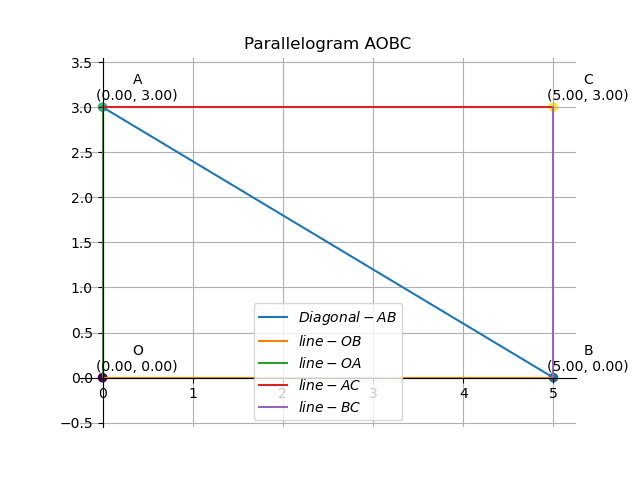
\includegraphics[width=0.6\linewidth]{figs/fig-1.png}
	\caption{The plot of the rectangle AOBC}
\end{figure}
\end{frame}
\begin{frame}[fragile]
\frametitle{C-Code}
\begin{minted}[bgcolor=bg, linenos, fontsize=\small, breaklines]{c}
#include <stdio.h>

// Function to calculate the C vertex
void find_c_vertex(double O[2], double A[2], double B[2], double C[2]) {
    C[0] = A[0] + B[0] - O[0];
    C[1] = A[1] + B[1] - O[1];
}}
//use this command gcc -shared -fPIC -o vertex.so vertex.c 
// to generate vertex.so lib
\end{minted}
\end{frame}
\begin{frame}[fragile]
  \frametitle{Python Code }

\begin{minted}[bgcolor=bg, linenos, fontsize=\tiny, breaklines]{python}
import sys                                          #for path to external scripts
sys.path.insert(0, '/home/koushik/matgeo/codes/CoordGeo')        #path to my scripts
import numpy as np
import numpy.linalg as LA
import matplotlib.pyplot as plt
import matplotlib.image as mpimg

#local imports
from line.funcs import *
from triangle.funcs import *
from conics.funcs import circ_gen

# Load the shared C library
lib = ctypes.CDLL('./vertex.so')

# Helper function to convert NumPy arrays to C arrays
def to_c_array(np_array):
    return (ctypes.c_double * 2)(*np_array)

# Define the Python function to call the C function
def calculate_c_vertex(O, A, B):
    C = (ctypes.c_double * 2)()  # Create an empty C array for the output (vertex C)

    # Convert NumPy arrays to C arrays using the helper function
    O_c = to_c_array(O)
    A_c = to_c_array(A)
    B_c = to_c_array(B)

    # Call the C function to calculate the vertex C
    lib.find_c_vertex(O_c, A_c, B_c, C)
\end{minted}
\end{frame}
\begin{frame}[fragile]
  \frametitle{Python Code }

\begin{minted}[bgcolor=bg, linenos, fontsize=\tiny, breaklines]{python}
 # Return the C vertex as a Python list
    return [C[0], C[1]]

# Generating points O, A, B
O = np.array([0, 0]).reshape(-1, 1)
B = np.array([5, 0]).reshape(-1, 1)
A = np.array([0, 3]).reshape(-1, 1)

# Call the function to calculate the fourth vertex C
C = np.array(calculate_c_vertex(O.flatten(), A.flatten(), B.flatten())).reshape(-1, 1)

# Generating lines for the parallelogram
from line.funcs import line_gen

x_OB = line_gen(O, B)
x_OA = line_gen(O, A)
x_BC = line_gen(B, C)
x_AC = line_gen(A, C)
x_AB = line_gen(A, B)

# Plotting the lines
plt.plot(x_AB[0,:], x_AB[1,:], label='$Diagonal-AB$')
plt.plot(x_OB[0,:], x_OB[1,:], label='$line-OB$')
plt.plot(x_OA[0,:], x_OA[1,:], label='$line-OA$')
plt.plot(x_AC[0,:], x_AC[1,:], label='$line-AC$')
plt.plot(x_BC[0,:], x_BC[1,:], label='$line-BC$')


\end{minted}
\end{frame}
\begin{frame}[fragile]
  \frametitle{Python Code }

\begin{minted}[bgcolor=bg, linenos, fontsize=\tiny, breaklines]{python}
# Labeling the coordinates
colors = np.arange(1, 5)
tri_coords = np.block([[O, B, A, C]])
plt.scatter(tri_coords[0,:], tri_coords[1,:], c=colors)
vert_labels = ['O', 'B', 'A', 'C']
for i, txt in enumerate(vert_labels):
    plt.annotate(f'{txt}\n({tri_coords[0,i]:.2f}, {tri_coords[1,i]:.2f})',
                 (tri_coords[0,i], tri_coords[1,i]),
                 textcoords="offset points",
                 xytext=(25, 5),
                 ha='center')

# Adjust plot aesthetics
ax = plt.gca()
ax.spines['top'].set_color('none')
ax.spines['left'].set_position('zero')
ax.spines['right'].set_color('none')
ax.spines['bottom'].set_position('zero')

plt.grid()
plt.axis('equal')
plt.title('Parallelogram AOBC')
plt.legend()
plt.show()

\end{minted}
\end{frame}
\end{document}
